\section{Sujet}

\subsection{L'interface}

L'interface d'OpenSCAD est composée de plusieurs fenêtres :


\begin{figure}[ht]
	\centering
	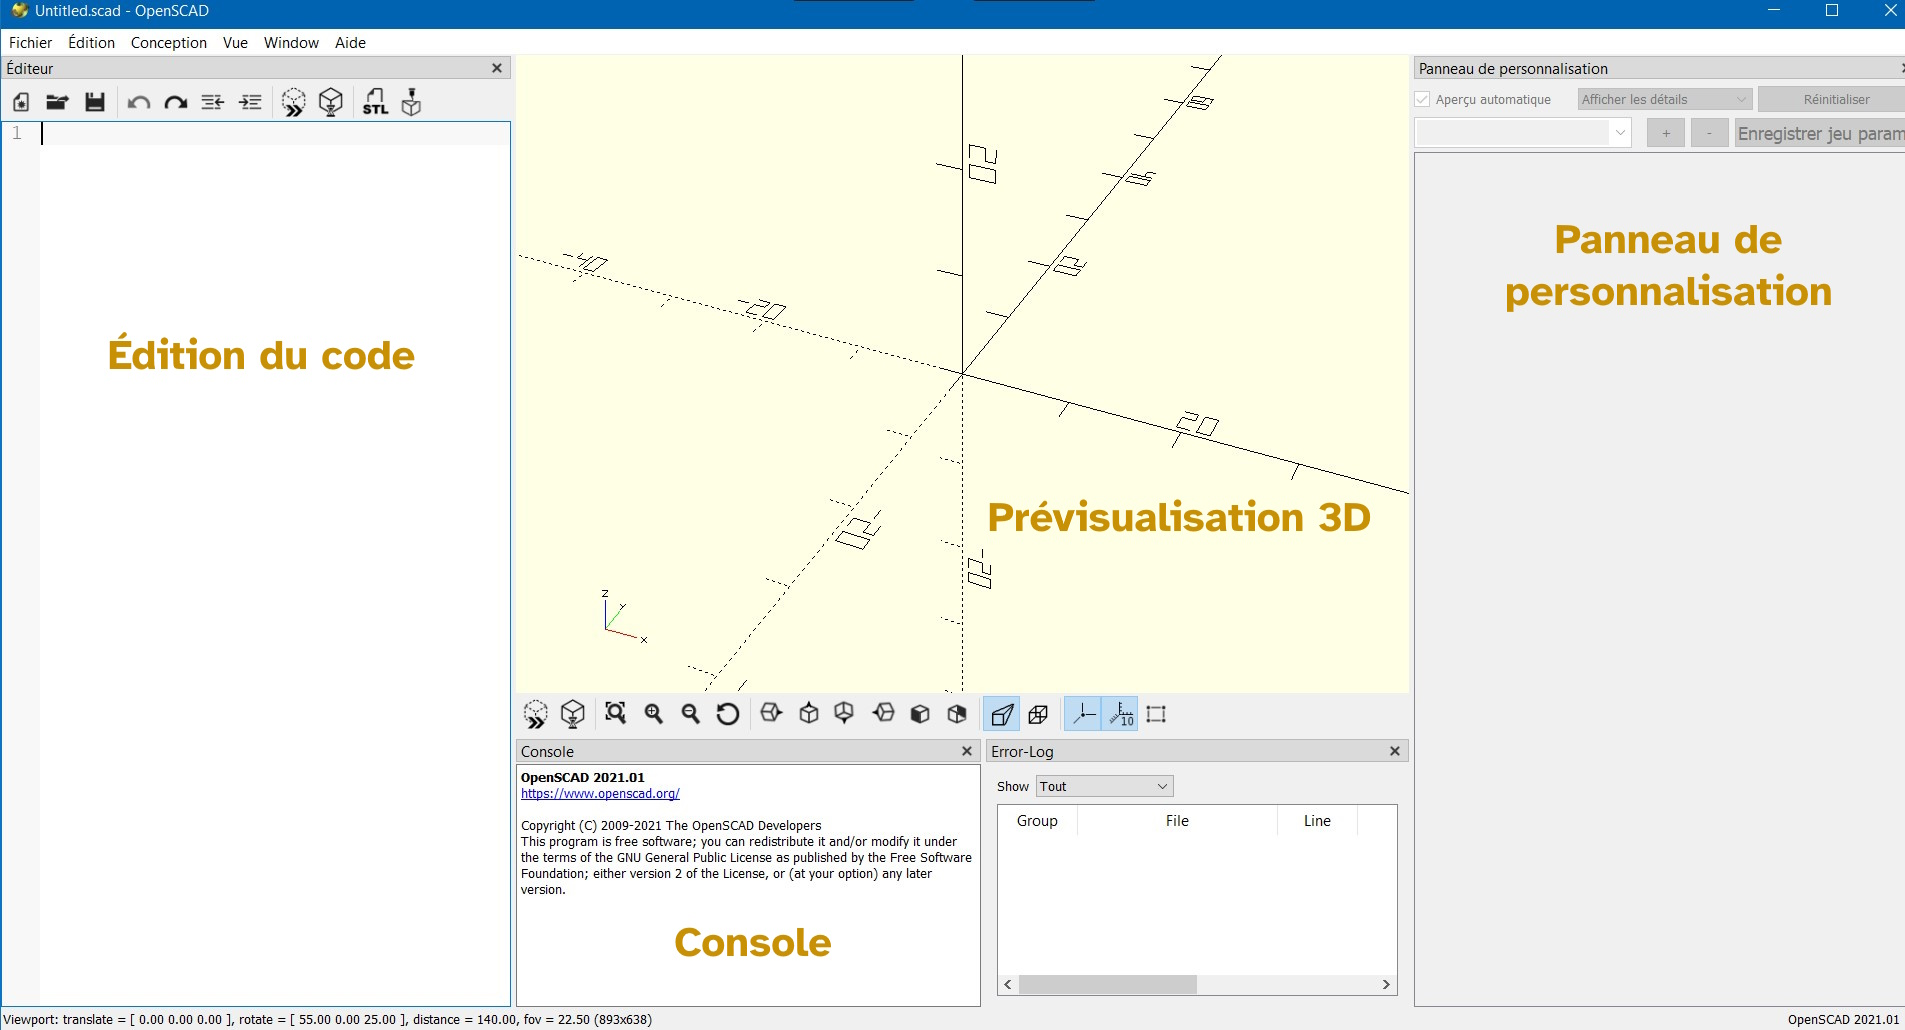
\includegraphics[width=12cm]{images/interface}
	\caption{\textit{Interface d'OpenSCAD}}
\end{figure}


\subsubsection{Éditeur}

C'est dans cette fenêtre que tout le code doit être écrit.
Le fonctionnement est semblable à n'importe quel éditeur classique, il faut rédiger le programme ligne par ligne, elles mêmes numérotées.
L'éditeur d'OpenSCAD fournit un système d'autocomplétion qui peut s'avérer très utile pour connaître rapidement la syntaxe attendue.


\subsubsection{Prévisualisation 3D}

Cette fenêtre permet de visualiser rapidement le rendu 3D décrit par le code.
Il n'est pas possible d'éditer directement les objets dans cette fenêtre.
Toutefois vous pouvez naviguer et explorer le modèle sous tous ses angles, afin de vérifier que le rendu correspond à vos attentes.

Vous pouvez modifier le thème de cette fenêtre en allant dans \textit{édition > préférences > vue 3D}.

Il est également possible de sélectionner les éléments que vous souhaitez voir dans la barre de boutons située au pied de la fenêtre.
Dans cette même barre, des boutons vous permettent de positionner la vue selon des orientations particulières (par exemple parfaitement au dessus du modèle).


\subsubsection{Console}

La console affiche les différentes informations lors de la compilation, le processus de transformation du code vers le modèle 3D.
Elle permet de voir les potentiels avertissements ou erreurs afin de les corriger.


\subsubsection{Panneau de personnalisation}

Nous n'utiliserons pas cette fenêtre dans cet atelier, elle est destinée à des utilisateurs avancés.


\subsection{Premiers pas}

\subsubsection{Formes basiques}

OpenSCAD dispose de plusieurs objets simples pour entamer la création de modèles : 
\verb|square|, \verb|circle|, \verb|cube|, \verb|cylinder| et \verb|sphere|.

Créons par exemple un cube d'1cm de côté. Pour cela il suffit d'écrire \verb|cube(1);| dans l'éditeur.
Ensuite, il faut appuyer sur la touche \verb|F5| de votre clavier pour pouvoir calculer l'aperçu.

\begin{figure}[ht]
	\centering
	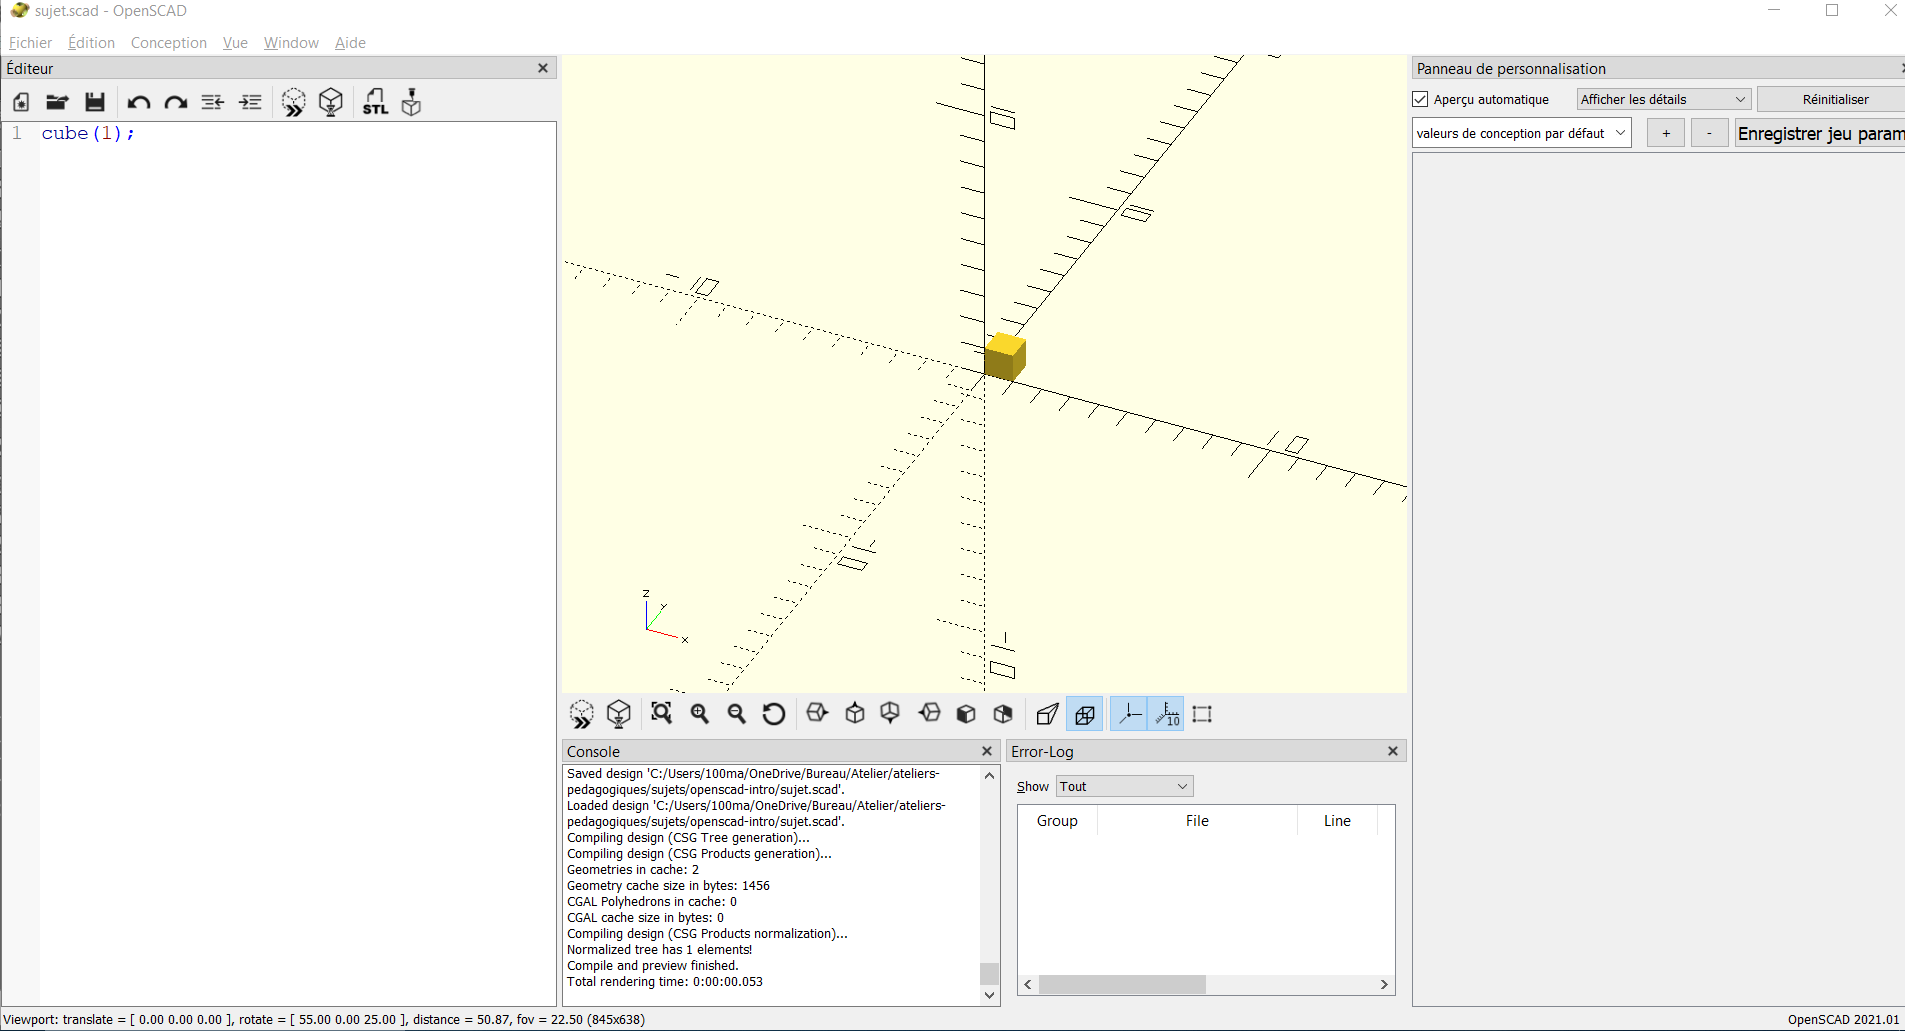
\includegraphics[width=12cm]{images/cube_1}
	\caption{\textit{Simple cube d'1cm de côté}}
\end{figure}

Rajoutons maintenant un pavé droit de 2cm de long, 2cm de large et 0.5cm de haut.
Cela se fait également avec la \textbf{fonction} \verb|cube| mais cette fois en mettant une liste de valeurs en \textbf{paramètre} : \verb|cube([2,2,0.5]);|.

\begin{figure}[ht]
	\centering
	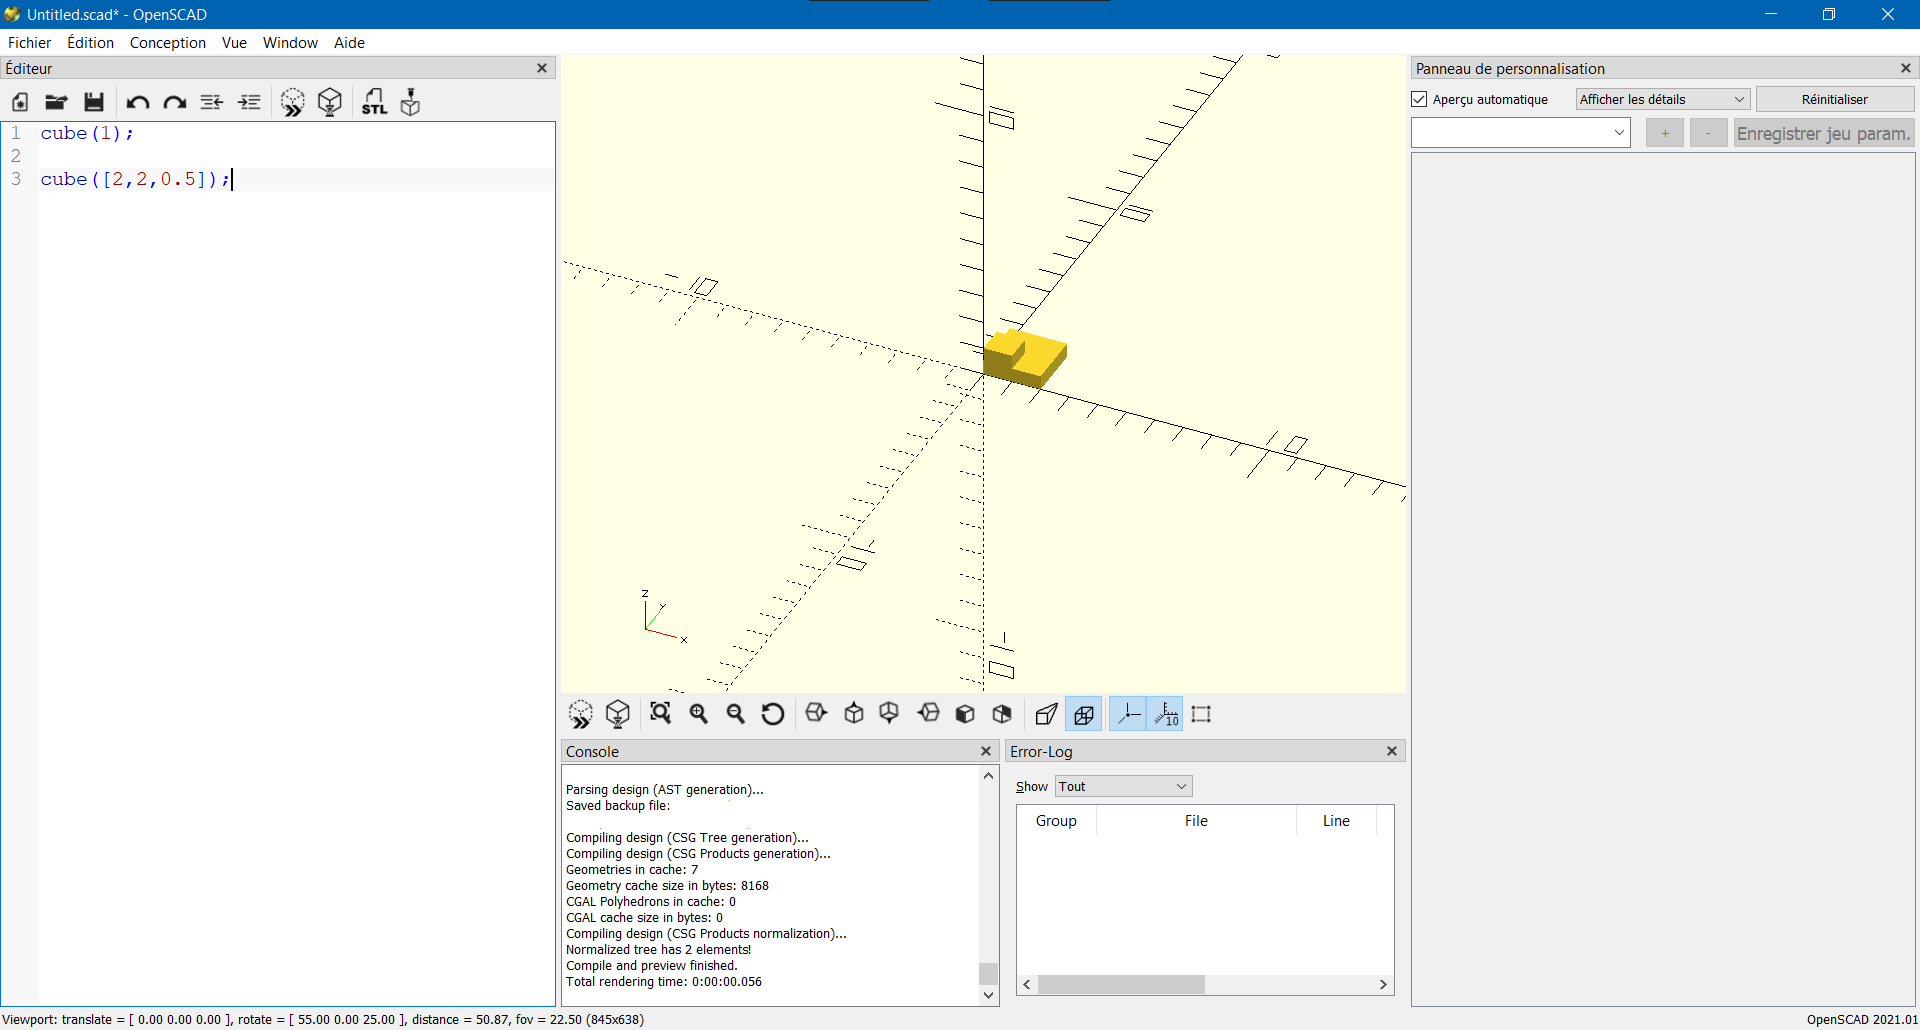
\includegraphics[width=12cm]{images/cube_2-2-05}
	\caption{\textit{Cube et Pavé droit}}
\end{figure}

\hint{
L'ordre des instructions est important. 
Ici, les dimensions sont notées selon l'axe x, puis l'axe y et enfin l'axe z.

Un repère est placé en bas à gauche de la fenêtre de visualisation.}

\warning{
Le langage d'OpenSCAD n'est pas \textit{indent sensitive}, c'est à dire que l'indentation (retours à la ligne et tabulations) ne change en rien l'exécution du programme.
Ainsi, afin de séparer les différents blocs d'instructions, il est nécessaire de mettre un \textbf{;} à la fin.
Sans ces points-virgules, le programme ne pourra pas compiler.}


\subsubsection{Transformations : translations}

Pour le moment, les objets que nous créons sont tous positionnés au même endroit dans l'espace, à partir de l'origine du repère.
Pour pouvoir les déplacer, nous allons appeler la fonction \verb|translate()|.

La syntaxe est la même que pour la création des objets, on indique les valeurs de translation dans une liste (entre crochets) dans l'ordre des axes.

\vspace{12pt}

\begin{figure}[ht]
	\centering
	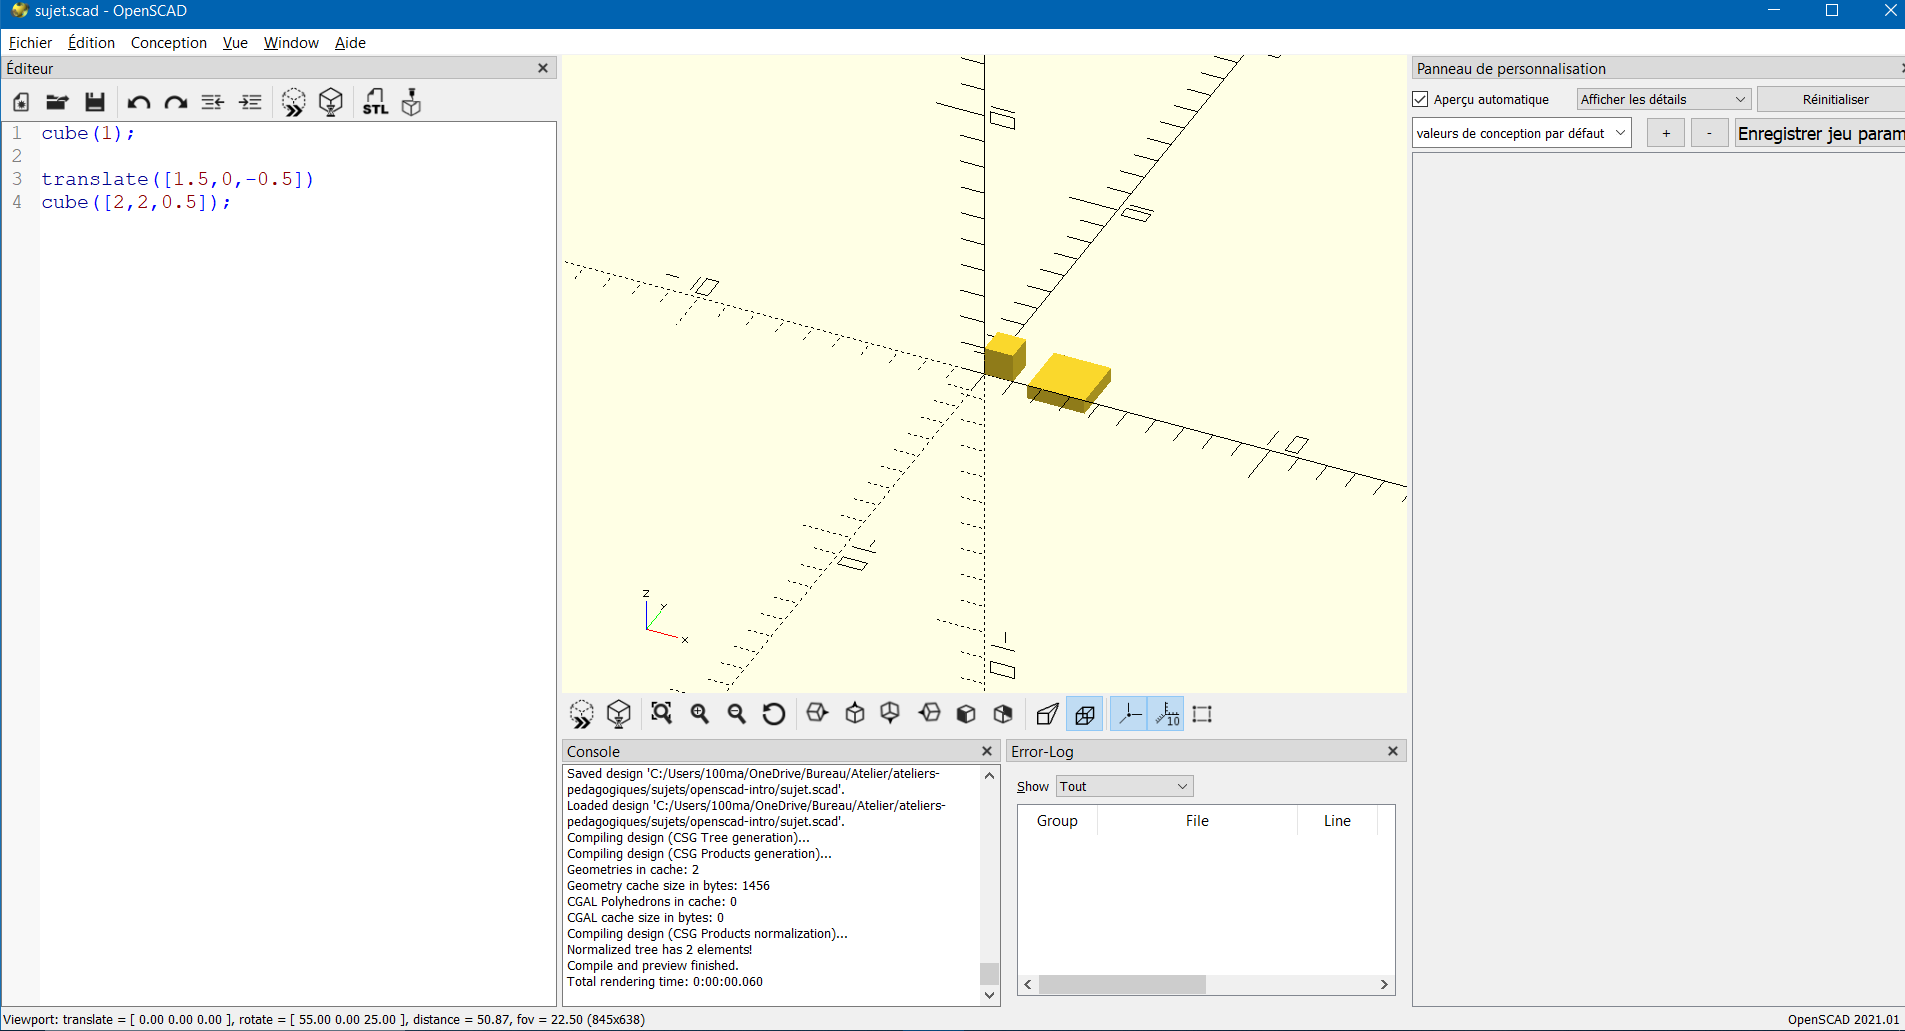
\includegraphics[width=12cm]{images/translate}
	\caption{\textit{Translation du pavé droit}}
\end{figure}

L'exemple suivant crée un cube d'1cm de côté, puis un pavé droit qui est translaté de 1.5 selon l'axe X et -0.5 selon l'axe Z.

La translation n'est appliquée qu'au deuxième objet car un point virgule a été mis après le premier cube.


\subsubsection{Transformations : rotations}

Nous avons comment effectuer des translations, passons désormais aux rotations.
Le fonctionnement est très similaire, il faut utiliser la fonction \verb|rotate()|.

\vspace{12pt}

\begin{figure}[ht]
	\centering
	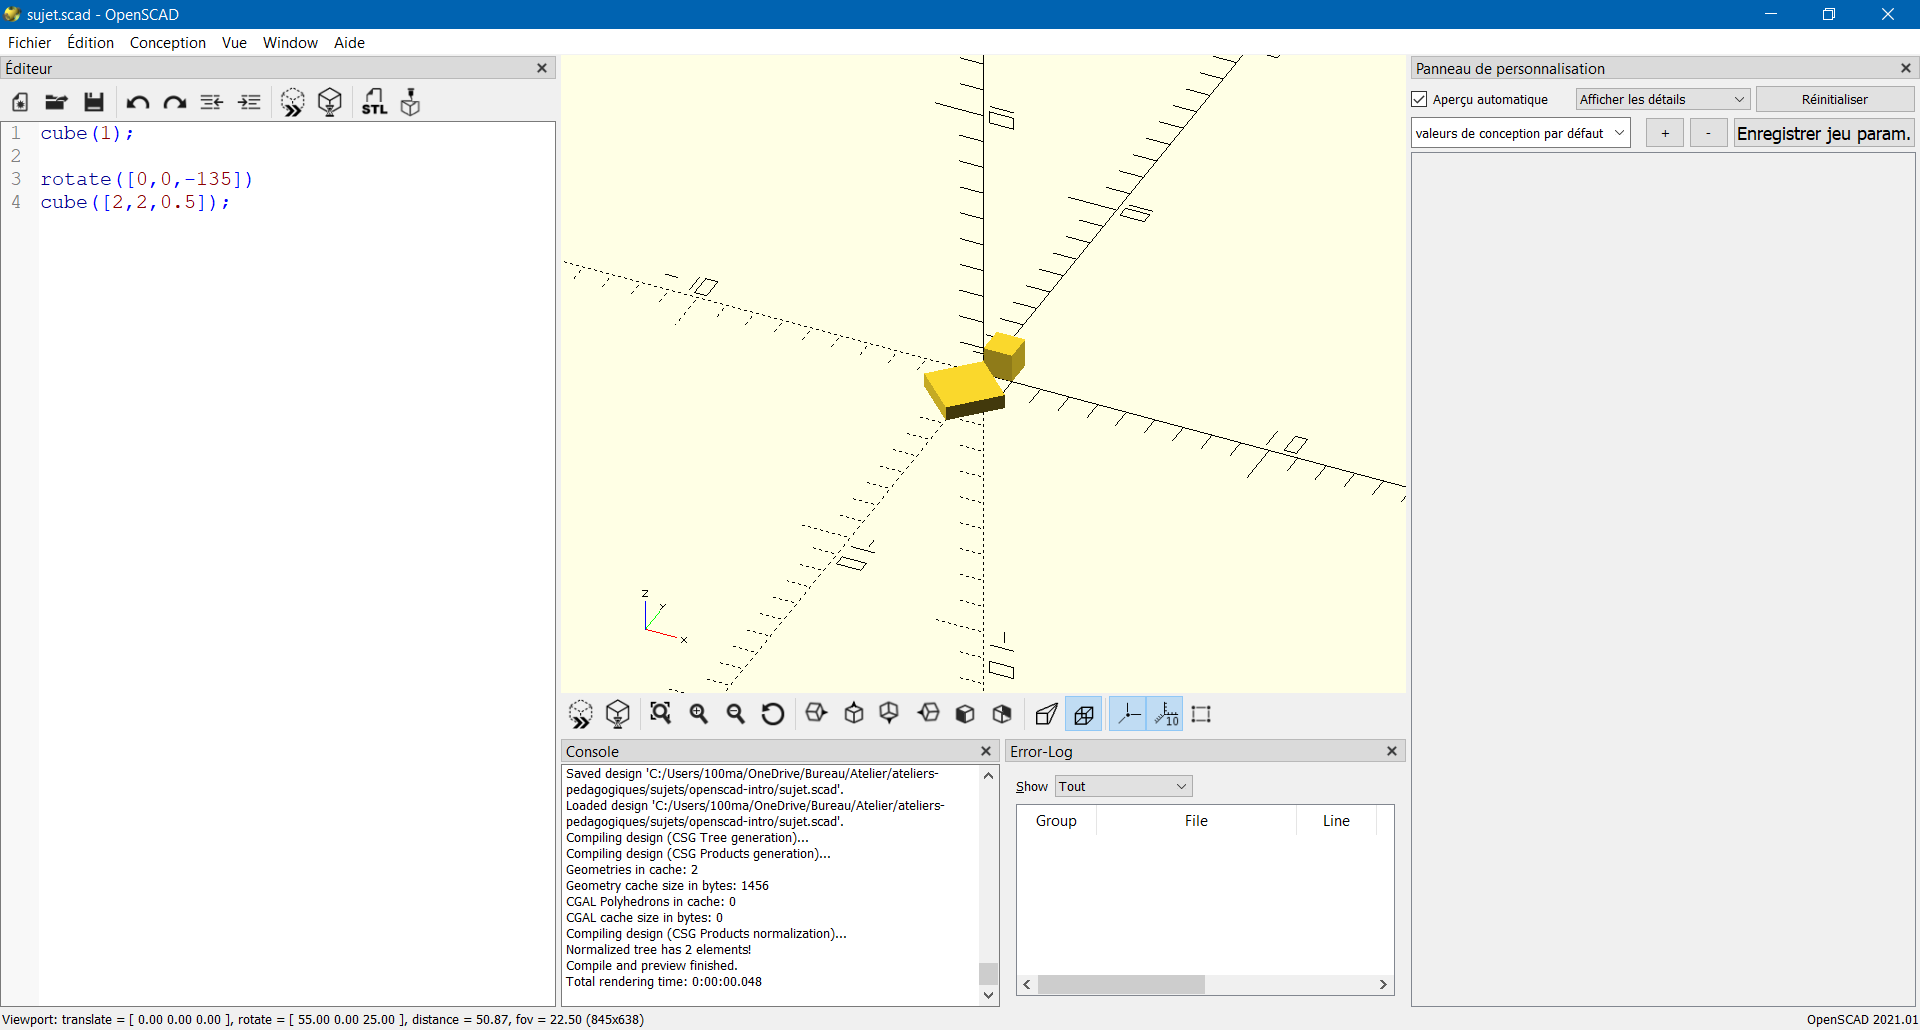
\includegraphics[width=12cm]{images/rotate}
	\caption{\textit{Rotation du pavé droit}}
\end{figure}

L'exemple suivant crée un cube d'1cm de côté, puis un pavé droit auquel est appliquée une rotation de -135° selon l'axe Z (vertical).


\subsubsection{Combinaison d'instructions}

Très souvent — voire quasiment tout le temps — il est nécessaire d'appliquer plusieurs modifications à un même objet. 
Pour cela, il suffit d'écrire les instructions les unes à la suite des autres.

Reprenons par exemple le même modèle (le cube et le pavé) et appliquons une rotation au pavé puis une translation.

\begin{figure}[ht]
	\centering
	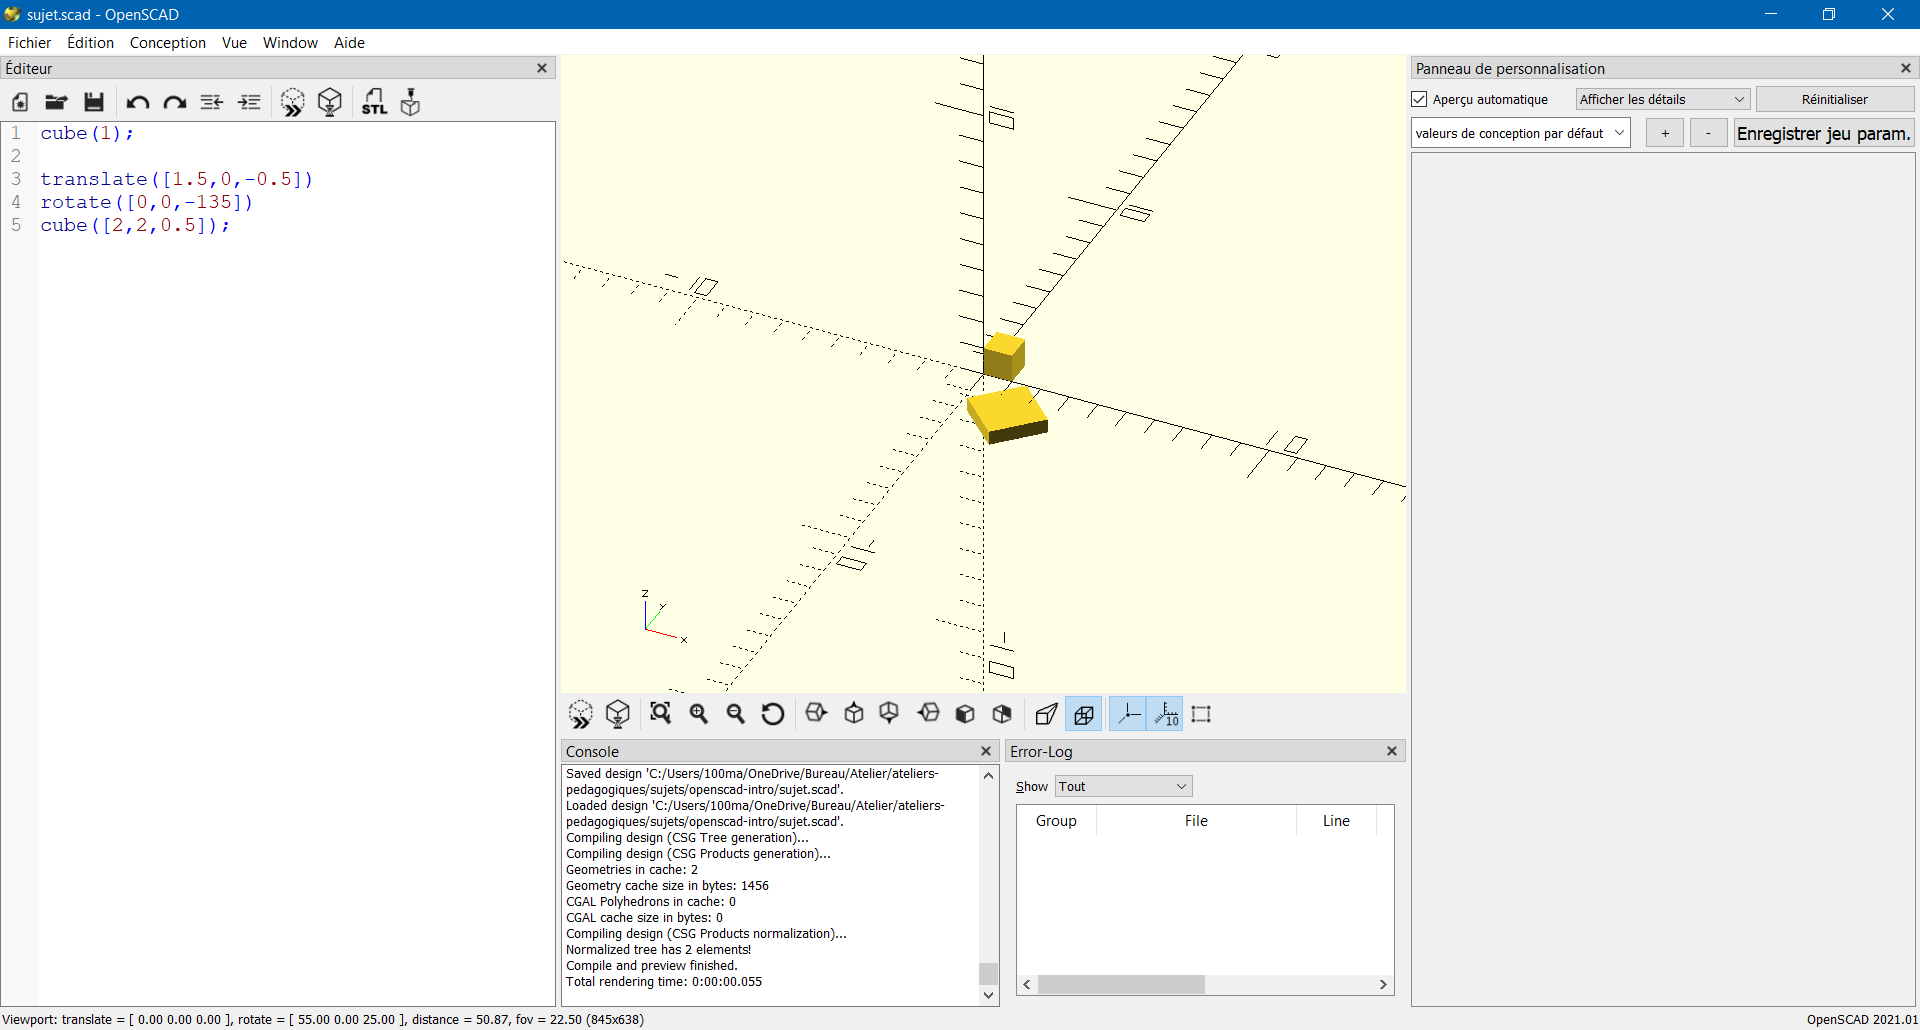
\includegraphics[width=12cm]{images/rotate-translate}
	\caption{\textit{Rotation puis translation du pavé droit}}
\end{figure}

\begin{figure}[ht]
	\centering
	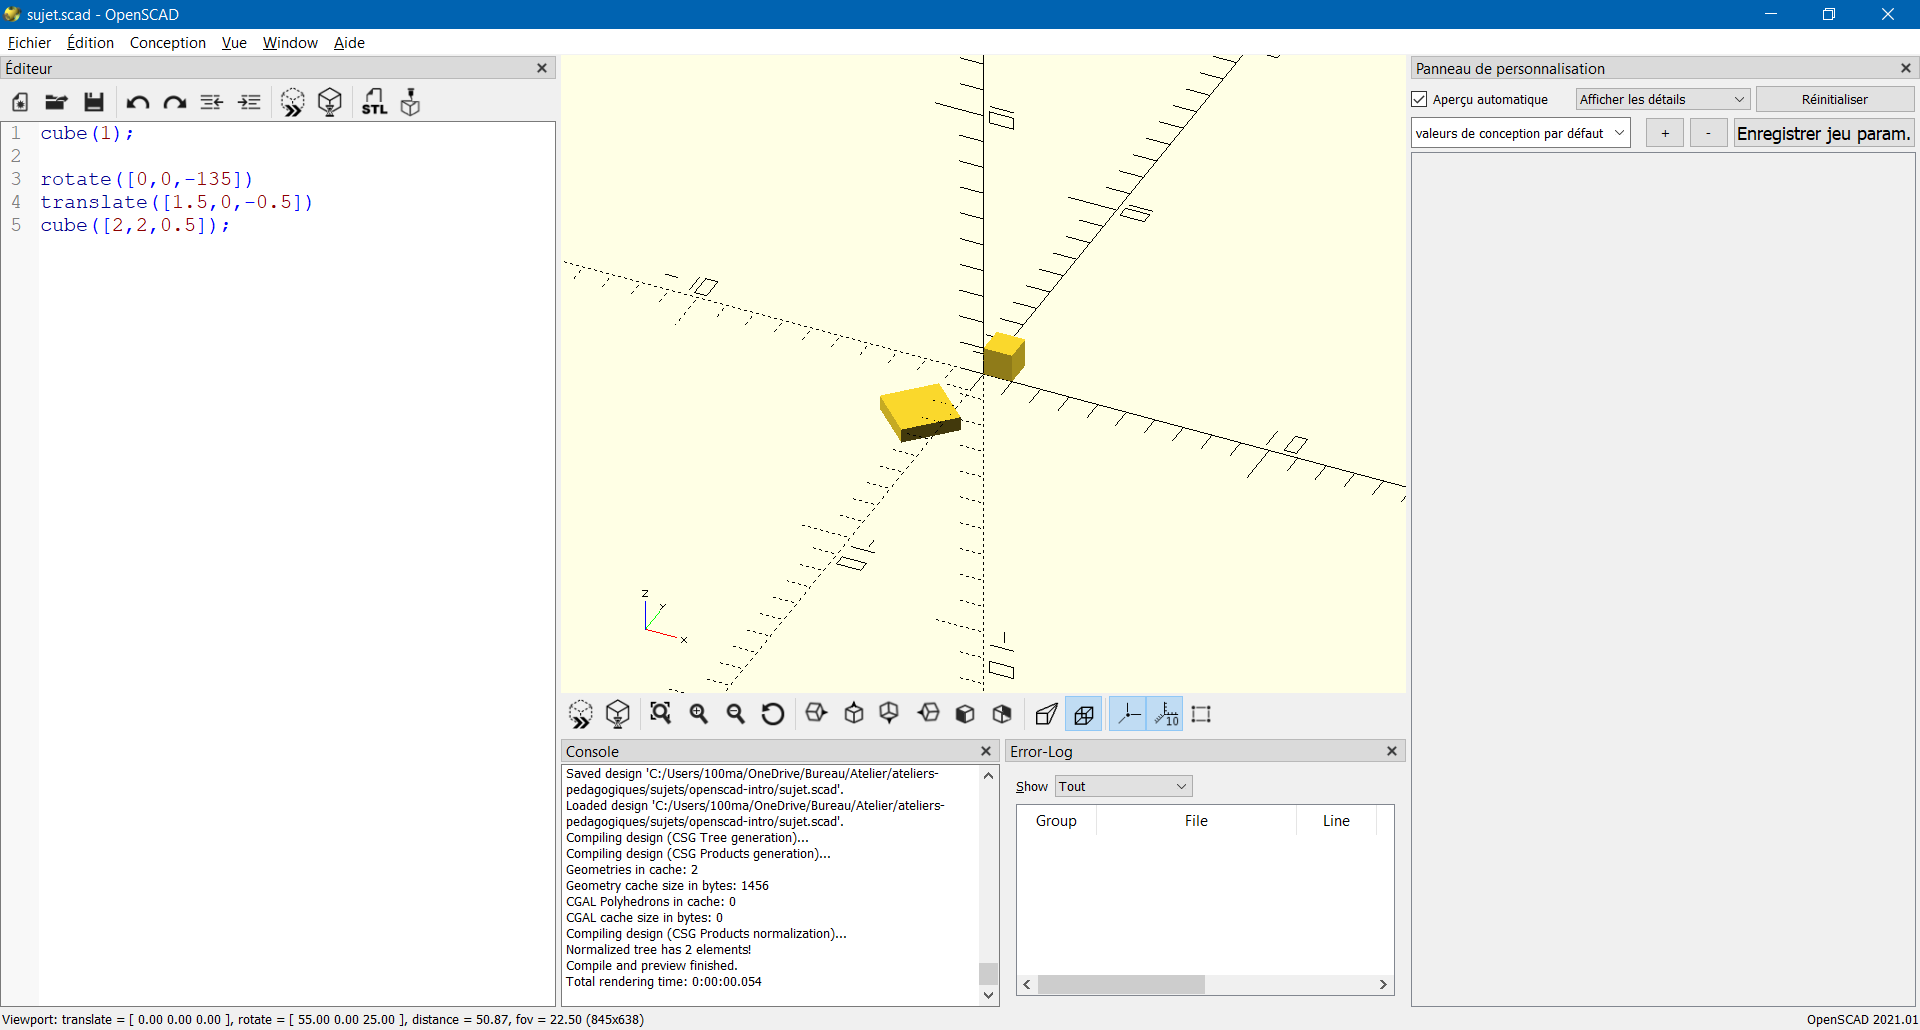
\includegraphics[width=12cm]{images/translate-rotate}
	\caption{\textit{Translation puis rotation du pavé droit}}
\end{figure}

\warning{
L'ordre des instructions est très important.
Il faut lire le code en le "remontant", c'est à dire en partant de la fin du bloc (souvent le modèle de base avec le point-virgule) puis en lisant à l'envers les instructions.

En effet, chaque nouvelle modification s'effectue sur le résultat de la précédente et non sur le modèle à l'origine.}